\documentclass[12pt,a4paper]{article}
\usepackage[utf8]{inputenc}
\usepackage[spanish]{babel}
\usepackage{amsmath}
\usepackage{amsfonts}
\usepackage{amssymb}
%\\usepackage[left=3cm,right=3cm,top=3cm,bottom=3cm]{geometry}		%para los márgenes
\usepackage{enumerate}	%para enumerar
\usepackage{lscape}		%para poner una página en horizontal
\usepackage{pdfpages}	%para incluir pdf
\usepackage{eurosym}		%para el símbolo del euro
\usepackage{emptypage}	%para que no aparezca encabezado en las páginas en blanco
\usepackage{fancyhdr}	%paquete para encabezado
\usepackage{lastpage}
\usepackage[hidelinks]{hyperref}		%para el índice con hipervínculos
\usepackage{float}
\usepackage{subfig}
\graphicspath{ {images/} }	%ruta de las imágenes



\cfoot{\thepage}
%\renewcommand{\headrulewidth}{0pt} 	%define el grosorde la línea

\begin{document}

% PORTADA
\begin{titlepage}
\begin{center}
% línea antes del título
\rule{80mm}{0.1mm}\\		%\rule{ancho}{alto}
\bigskip
% título de la portada
\begin{Huge}
\textsc{Genetic Tuning on Fuzzy Systems Based on the Linguistic 2-Tuples Representation\\}
\end{Huge}
% línea después del título
\bigskip
\rule{80mm}{0.1mm}\\		%\rule{ancho}{alto}
\bigskip

\includegraphics[scale=0.4]{Portada/logoUHU}\\
\bigskip
\bigskip
\Large
\textbf{Inteligencia computacional}\\
\bigskip
\bigskip
\bigskip
\bigskip
\bigskip
\bigskip
Profesor: Francisco Alfredo Márquez Hernández y Antonio Peregrín Rubio.\\
Alumnos: Ana Godoy Pérez y José Manuel Betanzos\\
\bigskip
\bigskip
\bigskip
Máster en Ingeniería Informática\\
Escuela Politécnica Superior de Ingeniería\\
Universidad de Huelva\\
\end{center}
\end{titlepage}


\thispagestyle{empty}
% ÍNDICE
\tableofcontents
%Cambiar nombre del indice
\renewcommand{\contentsname}{Índice}
%Indicar la profundidad
\setcounter{tocdepth}{3}
\newpage


% CONTENIDO
\part*{Objetivos}
El objetivo de esta práctica es la creación de un software que permita el diseño y lanzamiento de un controlador difuso MISO (Multiple input Simple Output) sobre un conjunto de valores de variables, que además permita un aprendizaje de las etiquetas lingüísticas (tuning) sobre un fichero de entrenamiento.

\section{Creación de un Software para el diseño y lanzamiento de un Controlador Difuso de Tipo Mamdani}
En esta primera parte se pretender crear un software que permita el diseño y lanzamiento de un controlador difuso de tipo Mandani. Este software permitirá definir el número de variables de entrada, la variable de salida, el universo de discurso, el número de etiquetas lingüísticas para cada una de las variables, así como el operador de implicación, conjunción y el método de inferencia. Además permitirá introducir una base de reglas en un formato
predefinido.
Para simplificar esta primera parte se utilizarán etiquetas triangulares. Además, como operadores de
conjunción e implicación la t-norma del mínimo y como método de defuzzificación un Modo B.

A continuación se van a explicar los paquetes de los que está compuesto este software, que se corresponden con los componentes forman un sistema difuso de este tipo: base de conocimiento, interfaz de fuzzificación, sistema de inferencia e interfaz de defuzzificación. Asímismo cuenta con otros paquetes auxiliares que ayudarán a cargar los datos necesarios en el sistema. Todos ellos cuenta con su JavaDoc y el código está comentado para facilitar la compresión del mismo.

También es necesario tener en consideración que la relación entre las partes del sistema será la mostrada en la siguiente imagen \ref{flujoFS} :
\begin{figure}[H]
\centering
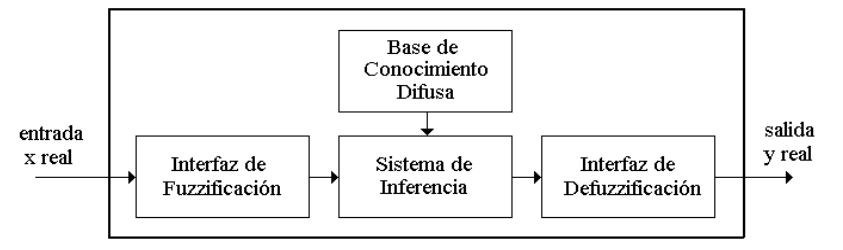
\includegraphics[width=0.8\textwidth]{flujoFS}
\caption{Flujo de un sistema difuso de tipo Mamdani.}
\label{flujoFS}
\end{figure}

\subsection{Base de conocimiento}
La base de conocimiento almacena el conocimiento particular del problema a resolver. Consta de dos elementos: la base de reglas y la base de conocimiento. Tanto la estructura de datos de la BC como la información que la formará debe ser especificada antes de que el SBRD comience a funcionar.

\begin{figure}[H]
\centering
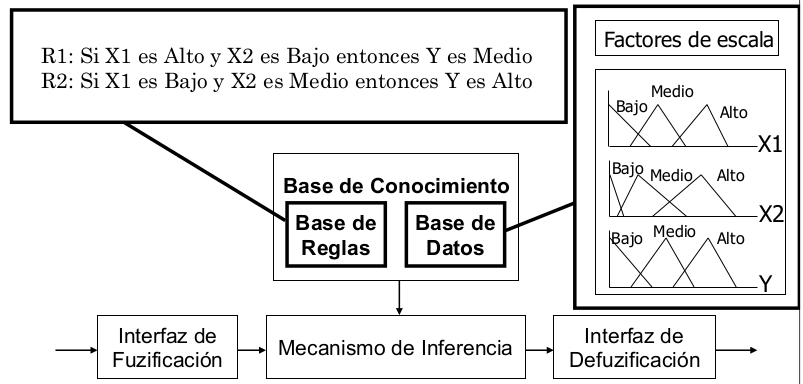
\includegraphics[width=0.8\textwidth]{baseConocimiento}
\caption{Base de conocimiento del sistema difuso.}
\label{flujoFS}
\end{figure}

\subsubsection{Base de Datos}
La base de datos contiene la definición de los conjuntos difusos asociados a los términos lingüísticos empleados en las reglas de la BR.\\
Para su definición se ha optado por una tabla hash en la que cada valor queda definido por el triángulo que representa a una partición difusa del conjunto difuso de las variables. Este ''triángulo'' no sólo almacena las coordenadas de la etiqueta si no que también almacena a qué variable del conjunto difuso pertenece. Como key de la tabla hash se empleará un número en el intervalo [1,num$\_$etiquetas].\\
Los datos necesarios para dar contenido a esta estructura serán tomados del fichero con extensión \textit{.pwm}

\subsubsection{Base de Reglas}
La base de reglas está formada por un conjunto de reglas lingüísticas de tipo ''Si - entonces''. En este caso las reglas contenidas en el fichero de extensión \textit{.wm} vienen definidas por las coordenadas de las etiquetas a las que hacen referencia.\\
Cada regla será almacenada como el conjunto de referencias a las etiquetas que la forman.

\subsection{Interfaz de fuzzificación}
Este componente es uno de los que permite al SBRD de tipo Mamdani manejar entradas y salidas reales. Su tarea es la de establecer una aplicación que haga corresponder un conjunto difuso, definido en el universo de discurso de la entrada en cuestión, a cada valor preciso del espacio de entrada.\\
Para almacenar esta correspondencia se ha optado de nuevo por una tabla hash que tendrá por clave la variable de entrada que se está considerando, y como valor las referencias a las particiones difusas (etiquetas) a las que pertenece.

\subsection{Sistema de inferencia}
El Sistema de Inferencia es el componente encargado de llevar a cabo el proceso de inferencia difusa. Para ello el Sistema de Inferencia deberá realizar las siguientes tareas sobre cada regla de la Base de Reglas:
\begin{itemize}
\item Determinar $\mu_{A}(x_{0})$, mediante el Operador de Conjunción (en esta práctica se empleará el mínimo).El resultado, denominado grado de emparejamiento (en adelante lo notaremos por h) de dichas entradas con la regla que se está evaluando, representa una medida de ''coincidencia'' de los valores que toman las variables de
entrada con los valores lingüísticos que describen el antecedente de esa regla. Estos valores se irán almacenando en el array \textit{matching} para su posterior uso.
\item Aplicar del Operador de Implicación, F (en esta práctica se empleará el mínimo). En el caso que nos ocupa, debido a que sólo existirá un consecuente, F = min, es decir, directamente se guardará el punto de máximo valor de la variable de salida del consecuente de la regla que se está evaluando en el vector \textit{pmv}.
\end{itemize}

\subsection{Interfaz de defuzzificación}
Convierte la salida del sistema de inferencia (lo inferido por cada regla) en un único valor real final. En este caso el método que se empleará para calcular este valor único será el Modo B, que consiste en convertir la aportación de cada regla en un número, que en esta práctica se ha hecho mediante el PMV (punto de máximo valor) y calcular un único valor final como salida empleando la siguiente fórmula: 
\begin{figure}[H]
\centering
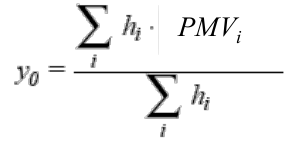
\includegraphics[width=0.3\textwidth]{salida}
\label{flujoFS}
\end{figure}

\subsection{Read}
Este paquete cuenta con las clases necesarias tanto para leer la información relativa al problema y almacenarla en  las estructuras correspondientes, como para escribir las salidas en el formato deseado.\\
A continuación se explica la finalidad de cada una de ellas:
\begin{itemize}
\item \textbf{ReadPWM:} lee un fichero de extensión .pwm que contiene la información relativa a la base de datos y la almacena.
\item \textbf{ReadRB:} lee un fichero de extensión .wm  que contiene las reglas que definen al sistema difuso. Este fichero también contiene la salida por defecto y el error cuadrático medio de los fichero tanto de training como de test.
\item \textbf{ReadExamples:} lee un fichero de training o test y guarda las entradas y salidas en dos estructuras respectivamente. Además esta clase permite calcular el error cuadrático medio del fichero leído, así como calcular las salidas para un conjunto de valores de entradas. También permite escribir las salidas obtenidas tras el entrenamiento o la fase de test siguiendo la estructura de estos ficheros.
\end{itemize}

\subsection{Files}
El paquete Files contiene los ficheros necesarios para la ejecución del sistema fuzzy: base de datos (.pwm), base de reglas (.wm), fichero de entrenamiento (.tra) y test (.tst). También albergará las salidas producidas tras una ejecución.

\subsection{FuzzySystem}
Este paquete contiene tanto la clase principal que contiene al \textit{main()}, como una clase en la que se han almacenado los parámetros que se emplearán a lo largo de todo el sistema.


\section{Ejecución del software}
Para ejecutar el software habrá que moverse a la carpeta \textit{FuzzySystem/dist}. Esta carpeta deberá contener el \textit{.jar} y la carpeta \textit{src/Files} con al menos los siguientes archivos: base de reglas, base de datos y fichero de entrenamiento. Además, esta carpeta contará con un README.TXT en el que se explica cómo ejecutar el software.\\
El controlador difuso se puede lanzar de dos formas:
\begin{itemize}
\item Dando un ejemplo de entrada, en cuyo caso devolverá la salida que quedará almacenada en \textit{src/Files/Output.txt}. La instrucción para ejecutar esta opción sería:\\
\begin{center}
\textit{java -jar "FuzzySystem.jar" -in valor1 valor2 valori}
\end{center}
\item Dando un fichero de entrenamiento \textit{.tra} con una secuencia de valores de entrada salida (una línea por cada secuencia), en cuyo caso cogerá por cada línea del fichero de entrenamiento los valores de las variables de entrada y devolverá los valores de la ejecución del controlador. Además, devolverá el error cuadrático medio (ECM). La salida de esta ejecución se almacenará en \textit{src/Files/Output$\_$tra.txt} siguiendo el mismo formato que el que tiene el fichero de entrenamiento. 
\begin{center}
\textit{java -jar FuzzySystem.jar -tra ruta$\_$del$\_$fichero.tra}
\end{center}
\end{itemize}


\end{document}


